\documentclass[conference]{IEEEtran}
\usepackage{cite}
\usepackage{amsmath,amssymb,amsfonts}
\usepackage{algorithmic}
\usepackage{graphicx}
\usepackage{textcomp}
\usepackage{array}
\usepackage{mathrsfs}
\usepackage{graphicx}
\usepackage{mathtools}
\def\BibTeX{{\rm B\kern-.05em{\sc i\kern-.025em b}\kern-.08em
    T\kern-.1667em\lower.7ex\hbox{E}\kern-.125emX}}
\begin{document}

\title{Deep Quaternion Networks}

\author{\IEEEauthorblockN{Chase J. Gaudet}
\IEEEauthorblockA{\textit{School of Computing \& Informatics} \\
\textit{University of Lousiana at Lafayette}\\
Lafayette, USA \\
cjg7182@louisiana.edu}
\and
\IEEEauthorblockN{Anthony S. Maida}
\IEEEauthorblockA{\textit{School of Computing \& Informatics} \\
\textit{University of Lousiana at Lafayette}\\
Lafayette, USA \\
maida@louisiana.edu}
}

\maketitle

\begin{abstract}
The field of deep learning has seen significant advancement in recent years.
However, much of the existing work has been focused on real-valued numbers.
Recent work has shown that a deep learning system using the complex numbers can be deeper for a fixed parameter budget compared to its real-valued counterpart.
In this work, we explore the benefits of generalizing one step further into the hyper-complex numbers, quaternions specifically, and provide the architecture components needed to build deep quaternion networks.
We go over quaternion convolutions, present a quaternion weight initialization scheme, and present algorithms for quaternion batch-normalization.
These pieces are tested in a classification model by end-to-end training on the CIFAR-10 and CIFAR-100 data sets and a segmentation model by end-to-end training on the KITTI Road Segmentation data set. 
The quaternion networks show improved convergence compared to real-valued and complex-valued networks, especially on the segmentation task.
\end{abstract}

\begin{IEEEkeywords}
quaternion, complex, neural networks, deep learning
\end{IEEEkeywords}

\section{Introduction}
There have been many advances in deep neural network architectures in the past few years.
One such improvement is a normalization technique called batch normalization \cite{ioffe2015batch} that standardizes the activations of layers inside a network using minibatch statistics.
It has been shown to regularize the network as well as provide faster and more stable training.
Another improvement comes from architectures that add so called shortcut paths to the network.
These shortcut paths connect later layers to earlier layers typically, which allows for the stronger gradients to propagate to the earlier layers.
This method can be seen in Highway Networks \cite{srivastava2015training} and Residual Networks  \cite{he2016deep}.
Other work has been done to find new activation functions with more desirable properties.
One example is the exponential linear unit (ELU) \cite{clevert2015fast}, which attempts to keep activations standardized.
All of the above methods are combating the vanishing gradient problem \cite{hochreiter1991untersuchungen} that plagues deep architectures.
With solutions to this problem appearing it is only natural to move to a system that will allow one to construct deeper architectures with as low a parameter cost as possible.

Other work in this area has explored the use of complex and hyper-complex numbers, which are a generalization of the complex, such as quaternions.
Using complex numbers in recurrent neural networks (RNNs) has been shown to increase learning speed and provide a more noise robust memory retrieval mechanism \cite{arjovsky2016unitary, danihelka2016associative, wisdom2016full}.
The first formulation of complex batch normalization and complex weight initialization is presented by \cite{trabelsi2017deep} where they achieve some state of the art results on the MusicNet data set.
Hyper-complex numbers are less explored in neural networks, but have seen use in manual image and signal processing techniques \cite{bulow1999hypercomplex, sangwine2000colour, bulow2001hypercomplex}.
Examples of using quaternion values in networks is mostly limited to architectures that take in quaternion inputs or predict quaternion outputs, but do not have quaternion weight values \cite{rishiyur2006neural, kendall2015posenet}. 
There are some more recent examples of building models that use quaternions represented as real-values. 
In \cite{parcollet2016quaternion} they used a quaternion multi-layer perceptron (QMLP) for document understanding and \cite{minemoto2017feed} uses a similar approach in processing multi-dimensional signals. 

Building on \cite{trabelsi2017deep} our contribution in this paper is to formulate and implement quaternion convolution, batch normalization, and weight initialization \footnote{Source code located at https://github.com/gaudetcj/DeepQuaternionNetworks}.
There arises some difficulty over complex batch normalization that we had to overcome as their is no analytic form for our inverse square root matrix.

\section{Motivation and Related Work}
The ability of quaternions to effectively represent spatial transformations and analyze multi-dimensional signals makes them promising for applications in artificial intelligence.

One common use of quaternions is for representing rotation into a more compact form. 
PoseNet \cite{kendall2015posenet} used a quaternion as the target output in their model where the goal was to recover the $6-$DOF camera pose from a single RGB image.
The ability to encode rotations may make a quaternion network more robust to rotational variance.

Quaternion representation has also been used in signal processing.  
The amount of information in the phase of an image has been shown to be sufficient to recover the majority of information encoded in its magnitude by Oppenheim and Lin \cite{oppenheim1981importance}.
The phase also encodes information such as shapes, edges, and orientations.
Quaternions can be represented as a 2~x~2 matrix of complex numbers, which gives them a group of phases potentially holding more information compared to a single phase.

Bulow and Sommer \cite{bulow2001hypercomplex} used the higher complexity representation of quaternions by extending Gabor's complex signal to a quaternion one which was then used for texture segmentation.
Another use of quaternion filters is shown in \cite{sangwine2000colour} where they introduce a new class of filter based on convolution with hyper-complex masks, and present three color edge detecting filters. 
These filters rely on a three-space rotation about the grey line of RGB space and when applied to a color image produce an almost greyscale image with color edges where the original image had a sharp change of color.
More quaternion filter use is shown in \cite{shi2007quaternion} where they show that it is effective in the context of segmenting color images into regions of similar color texture. 
They state the advantage of using quaternion arithmetic is that a color can be represented and analyzed as a single entity (by assigning each color channel to an imaginary axis), which we will see holds for quaternion convolution in a convolutional neural network architecture as well in Section \ref{s:qc}.

A quaternionic extension of a feed forward neural network, for processing multi-dimensional signals, is shown in \cite{minemoto2017feed}.
They expect that quaternion neurons operate on multi-dimensional signals as single entities, rather than real-valued neurons that deal with each element of signals independently.
A convolutional neural network (CNN) should be able to learn a powerful set of quaternion filters for more impressive tasks.

Another large motivation is discussed in \cite{trabelsi2017deep}, which is that complex numbers are more efficient and provide more robust memory mechanisms compared to the reals \cite{bulow1999hypercomplex, sangwine2000colour, bulow2001hypercomplex}.
They continue that residual networks have a similar architecture to associative memories since the residual shortcut paths compute their residual and then sum it into the memory provided by the identity connection.
Again, given that quaternions can be represented as a complex group, they may provide an even more efficient and robust memory mechanisms.


\section{Quaternion Network Components}
This section will include the work done to obtain a working deep quaternion network. 
Some of the longer derivations are given in the Appendix.

\subsection{Quaternion Representation}
In 1833 Hamilton proposed complex numbers $\mathbb{C}$ be defined as the set $\mathbb{R}^2$ of ordered pairs $(a, b)$ of real numbers.
He then began working to see if triplets $(a,b,c)$ could extend multiplication of complex numbers.
In 1843 he discovered a way to multiply in four dimensions instead of three, but the multiplication lost commutativity.
This construction is now known as quaternions.
Quaternions are composed of four components, one real part, and three imaginary parts.
Typically denoted as
\begin{equation}
\mathbb{H} = \{a + b\textit{i} + c\textit{j} + d\textit{k}~:~a,b,c,d \in \mathbb{R}\}
\label{eq:quaternion1}
\end{equation}
where $a$ is the real part, $(i,j,k)$ denotes the three imaginary axis, and $(b,c,d)$ denotes the three imaginary components.
Quaternions are governed by the following arithmetic:
\begin{equation}
i^2=j^2=k^2=ijk=-1
\label{eq:quarternion2}
\end{equation}
which, by enforcing distributivity, leads to the noncommutative multiplication rules
\begin{equation}
ij=k,~jk=i,~ki=j,~ji=-k,~kj=-i,~ik=-j
\label{eq:quarternion3}
\end{equation}

Since we will be performing quaternion arithmetic using reals it is useful to embed $\mathbb{H}$ into a real-valued representation.
There exists an injective homomorphism from $\mathbb{H}$ to the matrix ring $M(4,\mathbb{R})$ where $M(4,\mathbb{R})$ is a 4x4 real matrix.
The 4~x~4 matrix can be written as
\begin{align}
\begin{bmatrix}
 a & -b & -c & -d \\ 
 b & a & -d & c \\
 c & d & a & -b \\
 d & -c & b & a 
\end{bmatrix}= &~~a
\begin{bmatrix}
 1 & 0 & 0 & 0 \\ 
 0 & 1 & 0 & 0 \\
 0 & 0 & 1 & 0 \\
 0 & 0 & 0 & 1 
\end{bmatrix}
\nonumber \\ &+ b 
\begin{bmatrix}
 0 & -1 & 0 & 0 \\ 
 1 & 0 & 0 & 0 \\
 0 & 0 & 0 & -1 \\
 0 & 0 & 1 & 0 
\end{bmatrix}
\nonumber \\ &+ c
\begin{bmatrix}
 0 & 0 & -1 & 0 \\ 
 0 & 0 & 0 & 1 \\
 1 & 0 & 0 & 0 \\
 0 & -1 & 0 & 0 
\end{bmatrix}
\nonumber \\ &+ d
\begin{bmatrix}
 0 & 0 & 0 & -1 \\ 
 0 & 0 & -1 & 0 \\
 0 & 1 & 0 & 0 \\
 1 & 0 & 0 & 0 
\end{bmatrix}.
\label{eq:m4r}
\end{align}
This representation of quaternions is not unique, but we will stick to the above in this paper.
It is also possible to represent $\mathbb{H}$ as $M(2,\mathbb{C})$ where $M(2,\mathbb{C})$ is a 2~x~2 complex matrix.

With our real-valued representation a quaternion real-valued $2D$ convolution layer can be expressed as follows. 
Say that the layer has $N$ feature maps such that $N$ is divisible by 4.
We let the first $N/4$ feature maps represent the real components, the second $N/4$ represent the $i$ imaginary components, the third $N/4$ represent the $j$ imaginary components, and the last $N/4$ represent the $k$ imaginary components.


\subsection{Quaternion Differentiability}
In order for the network to perform backpropagation the cost function and activation functions used must be differentiable with respect to the real, $i$, $j$, and $k$ components of each quaternion parameter of the network.
As the complex chain rule is shown in \cite{trabelsi2017deep}, we provide the quaternion chain rule which is given in the Appendix section \ref{a:diff}.


\subsection{Quaternion Convolution}\label{s:qc}
Convolution in the quaternion domain is done by convolving a quaternion filter matrix $\textbf{W}=\textbf{A}+\textit{i}\textbf{B}+\textit{j}\textbf{C}+\textit{k}\textbf{D}$ by a quaternion vector $\textbf{h}=\textbf{w}+\textit{i}\textbf{x}+\textit{j}\textbf{y}+\textit{k}\textbf{z}$. 
Performing the convolution by using the distributive property and grouping terms one gets
\begin{align}
\textbf{W}\ast \textbf{h} = &~(\textbf{A}\ast\textbf{w}-\textbf{B}\ast\textbf{x}-\textbf{C}\ast\textbf{y}-\textbf{D}\ast\textbf{z}) + \nonumber \\ 
&\textit{i}(\textbf{A}\ast\textbf{x}+\textbf{B}\ast\textbf{w}+\textbf{C}\ast\textbf{z}-\textbf{D}\ast\textbf{y}) + \nonumber \\
&\textit{j}(\textbf{A}\ast\textbf{y}-\textbf{B}\ast\textbf{z}+\textbf{C}\ast\textbf{w}+\textbf{D}\ast\textbf{x}) + \nonumber \\
&\textit{k}(\textbf{A}\ast\textbf{z}+\textbf{B}\ast\textbf{y}-\textbf{C}\ast\textbf{x}+\textbf{D}\ast\textbf{w}).
\label{eq:convolve1}
\end{align}
Using a matrix to represent the components of the convolution we have:
\begin{equation}
\begin{bmatrix}
 \mathscr{R}(\textbf{W}\ast \textbf{h}) \\ 
 \mathscr{I}(\textbf{W}\ast \textbf{h}) \\
 \mathscr{J}(\textbf{W}\ast \textbf{h}) \\
 \mathscr{K}(\textbf{W}\ast \textbf{h}) 
\end{bmatrix}
=
\begin{bmatrix}
 \textbf{A} & -\textbf{B} & -\textbf{C} & -\textbf{D}\\
 \textbf{B} & \textbf{A} & -\textbf{D} & \textbf{C} \\
 \textbf{C} & \textbf{D} & \textbf{A} & -\textbf{B} \\
 \textbf{D} & -\textbf{C} & \textbf{B} & \textbf{A} \\
\end{bmatrix}
\ast
\begin{bmatrix}
 \textbf{w} \\ 
 \textbf{x} \\
 \textbf{y} \\
 \textbf{z}
\end{bmatrix}
\label{eq:}
\end{equation}
An example is shown in Fig.~\ref{f:quatconv} where one can see how quaternion convolution forces a linear depthwise mixture of the channels. This is similar to a mixture of standard convolution and depthwise separable convolution from \cite{chollet2016xception}. This reuse of filters on every layer and combination may help extract texture information across channels as seen in \cite{shi2007quaternion}.

\begin{figure*}
	\centering
		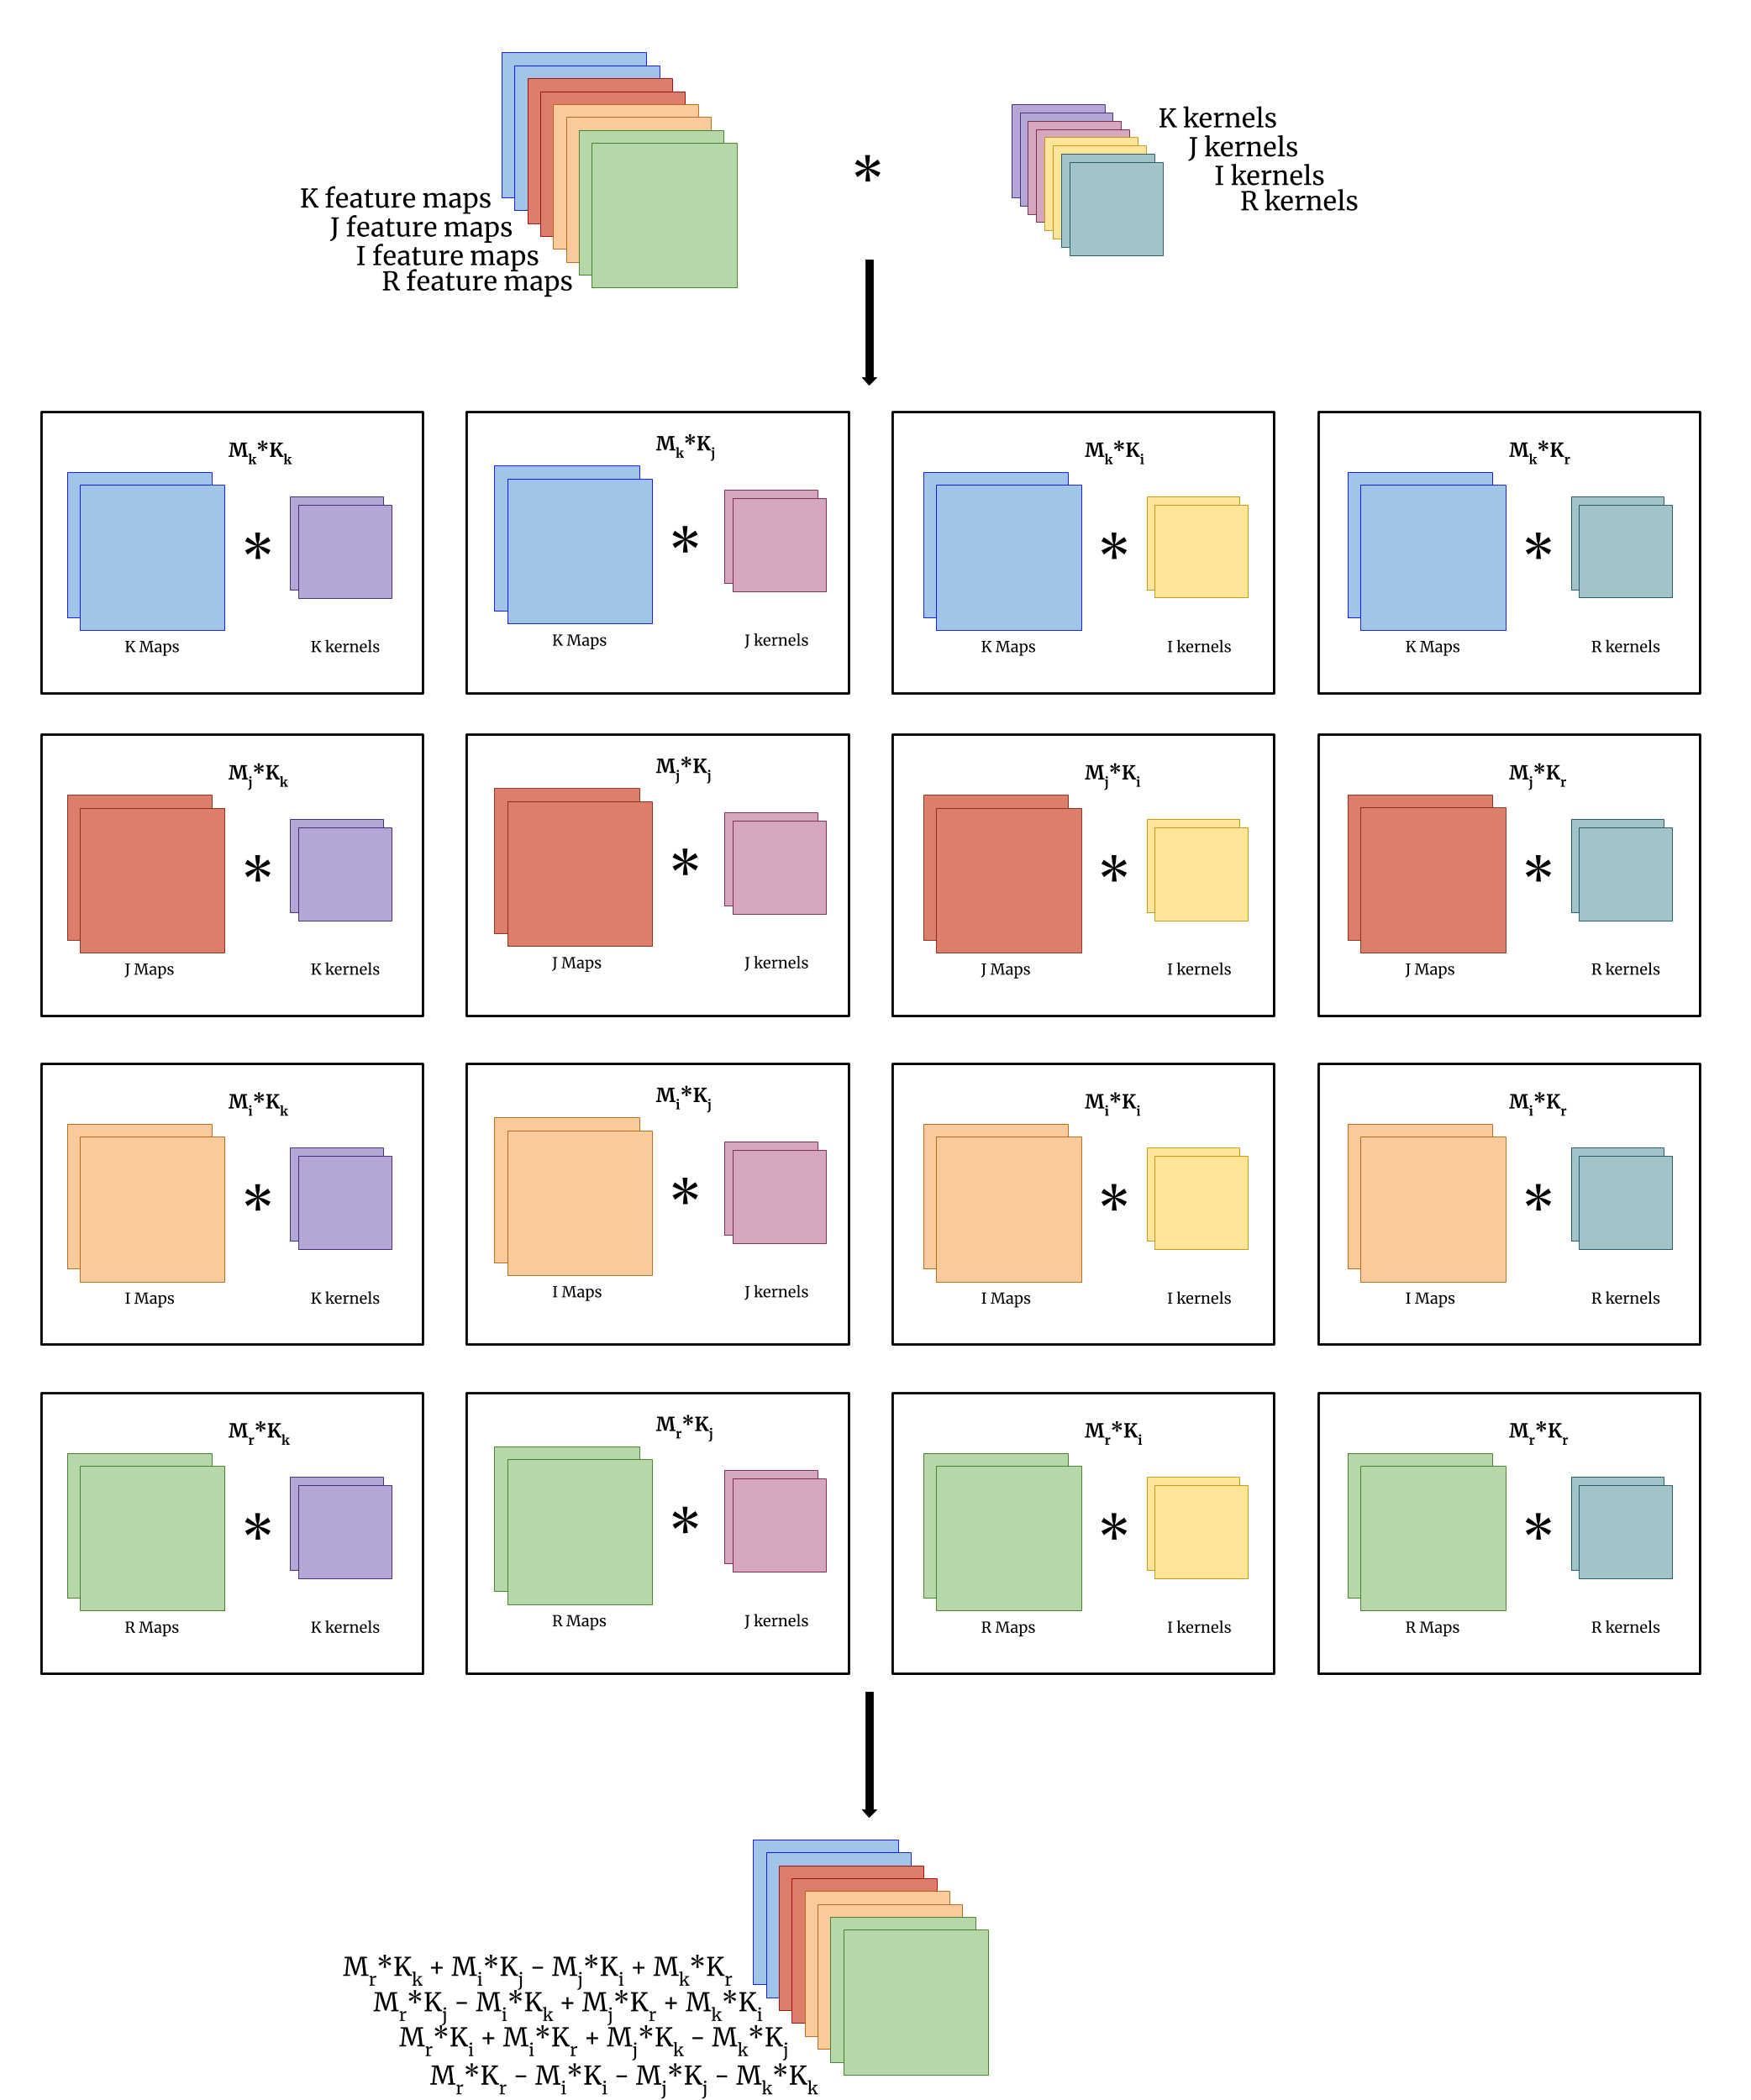
\includegraphics[width=1.0\textwidth]{quatconv.png}
	\caption{An illustration of quaternion convolution.}
	\label{f:quatconv}
\end{figure*}


\subsection{Quaternion Batch-Normalization}
Batch-normalization \cite{ioffe2015batch} is used by the vast majority of all deep networks to stabilize and speed up training.
It works by keeping the activations of the network at zero mean and unit variance.
The original formulation of batch-normalization only works for real-values. 
Applying batch normalization to complex or hyper-complex numbers is more difficult, one can not simply translate and scale them such that their mean is 0 and their variance is 1.
This would not give equal variance in the multiple components of a complex or hyper-complex number.
To overcome this for complex numbers a whitening approach is used \cite{trabelsi2017deep}, which scales the data by the square root of their variances along each of the two principle components.
We use the same approach, but must whiten 4D vectors.

However, an issue arises in that there is no nice way to calculate the inverse square root of a 4~x~4 matrix.
It turns out that the square root is not necessary and we can instead use the Cholesky decomposition on our covariance matrix.
The details of why this works for whitening given in the Appendix section \ref{a:whitening}.
Now our whitening is accomplished by multiplying the \textbf{0}-centered data ($\textbf{x} - \mathbb{E}[\textbf{x}]$) by \textbf{W}:
\begin{equation}
\tilde{x} = \textbf{W}(\textbf{x} - \mathbb{E}[\textbf{x}])
\label{eq:white4d}
\end{equation}
where \textbf{W} is one of the matrices from the Cholesky decomposition of $\textbf{V}^{-1}$ where \textbf{V} is the covariance matrix given by:
\begin{align}
\textbf{V}
=&
\begin{bmatrix}
 V_{rr} & V_{ri} & V_{rj} & V_{rk} \\
 V_{ir} & V_{ii} & V_{ij} & V_{ik} \\
 V_{jr} & V_{ji} & V_{jj} & V_{jk} \\
 V_{kr} & V_{ki} & V_{kj} & V_{kk}
\end{bmatrix} \nonumber \\
=&~~  \left[ 
\begin{matrix*}[l]
\mbox{Cov}(\mathscr{R}\{\textbf{x}\}, \mathscr{R}\{\textbf{x}\}) \\
\mbox{Cov}(\mathscr{I}\{\textbf{x}\}, \mathscr{R}\{\textbf{x}\}) \\
\mbox{Cov}(\mathscr{J}\{\textbf{x}\}, \mathscr{R}\{\textbf{x}\}) \\
\mbox{Cov}(\mathscr{K}\{\textbf{x}\}, \mathscr{R}\{\textbf{x}\}) \\
\end{matrix*} \right. \nonumber \\ 
&~~~~~~
\begin{matrix*}[l]
\mbox{Cov}(\mathscr{R}\{\textbf{x}\}, \mathscr{I}\{\textbf{x}\}) \\
\mbox{Cov}(\mathscr{I}\{\textbf{x}\}, \mathscr{I}\{\textbf{x}\}) \\
\mbox{Cov}(\mathscr{J}\{\textbf{x}\}, \mathscr{I}\{\textbf{x}\}) \\
\mbox{Cov}(\mathscr{K}\{\textbf{x}\}, \mathscr{I}\{\textbf{x}\}) \\
\end{matrix*} \nonumber \\
&~~~~~~~
\begin{matrix*}[l]
\mbox{Cov}(\mathscr{R}\{\textbf{x}\}, \mathscr{J}\{\textbf{x}\}) \\
\mbox{Cov}(\mathscr{I}\{\textbf{x}\}, \mathscr{J}\{\textbf{x}\}) \\
\mbox{Cov}(\mathscr{J}\{\textbf{x}\}, \mathscr{J}\{\textbf{x}\}) \\
\mbox{Cov}(\mathscr{K}\{\textbf{x}\}, \mathscr{J}\{\textbf{x}\}) \\
\end{matrix*} \nonumber \\
&~~~~~~~~ \left.
\begin{matrix*}[l]
\mbox{Cov}(\mathscr{R}\{\textbf{x}\}, \mathscr{K}\{\textbf{x}\}) \\
\mbox{Cov}(\mathscr{I}\{\textbf{x}\}, \mathscr{K}\{\textbf{x}\}) \\
\mbox{Cov}(\mathscr{J}\{\textbf{x}\}, \mathscr{K}\{\textbf{x}\}) \\
\mbox{Cov}(\mathscr{K}\{\textbf{x}\}, \mathscr{K}\{\textbf{x}\}) \\
\end{matrix*}  \right]
\label{eq:V4d}
\end{align}
where Cov$(\cdot)$ is the covariance and $\mathscr{R}\{x\}$, $\mathscr{I}\{x\}$, $\mathscr{J}\{x\}$, and $\mathscr{K}\{x\}$ are the real, $i$, $j$, and $k$ components of $\textbf{x}$ respectively.

Real-valued batch normalization also uses two learned parameters, $\beta$ and $\gamma$. 
Our shift parameter {\boldmath$\beta$} must shift a quaternion value so it is a quaternion value itself with real, $i$, $j$, and $k$ as learnable components. 
The scaling parameter {\boldmath$\gamma$} is a symmetric matrix of size matching $\textbf{V}$ given by:
\begin{equation}
\mathbf{\gamma}
=
\left( 
\begin{array}{cccc}
\gamma_{rr} & \gamma_{ri} & \gamma_{rj} & \gamma_{rk} \\
\gamma_{ri} & \gamma_{ii} & \gamma_{ij} & \gamma_{ik} \\
\gamma_{rj} & \gamma_{ij} & \gamma_{jj} & \gamma_{jk} \\
\gamma_{rk} & \gamma_{ik} & \gamma_{jk} & \gamma_{kk}
\end{array}
\right)
\label{eq:gamma}
\end{equation}
Because of its symmetry it has only ten learnable parameters. 
The variance of the components of input $\tilde{\textbf{x}}$ are variance 1 so the diagonal of {\boldmath$\gamma$} is initialized to $1/\sqrt{4}$ in order to obtain a modulus of 1 for the variance of the normalized value. 
The off diagonal terms of {\boldmath$\gamma$} and all components of {\boldmath$\beta$} are initialized to 0.
The quaternion batch normalization is defined as:
\begin{equation}
\mbox{BN}(\tilde{\textbf{x}}) = \mathbf{\gamma}\tilde{\textbf{x}} + \mathbf{\beta}
\label{eq:qbn}
\end{equation}


\subsection{Quaternion Weight Initialization}
The proper initialization of weights is vital to convergence of deep networks. 
In this work we derive our quaternion weight initialization using the same procedure as Glorot and Bengio \cite{glorot2010understanding} and He et al. \cite{he2015delving}.

To begin we find the variance of a quaternion weight:
\begin{align}
W = &~|W|e^{(\mbox{cos}\phi_1 \textit{i} + \mbox{cos}\phi_2 \textit{j} + \mbox{cos}\phi_3 \textit{k})\theta} \nonumber \\
= &~\mathscr{R}\{W\} + i~\mathscr{I}\{W\} + j~\mathscr{J}\{W\} + k~\mathscr{K}\{W\}.
\label{eq:quaternion_weight}
\end{align}
where $|W|$ is the magnitude, $\theta$ and $\phi$ are angle arguments, and $\mbox{cos}^2\phi_1 + \mbox{cos}^2\phi_2 + \mbox{cos}^2\phi_3 = 1$ \cite{turner2002}.

Variance is defined as
\begin{equation}
\mbox{Var}(W) = \mathbb{E}[|W|^2] - (\mathbb{E}[W])^2,
\label{eq:variance}
\end{equation}
but since $W$ is symmetric around 0 the term $(\mathbb{E}[W])^2$ is 0. 
We do not have a way to calculate $\mbox{Var}(W) = \mathbb{E}[|W|^2]$ so we make use of the magnitude of quaternion normal values $|W|$, which follows an independent normal distribution with four degrees of freedom (DOFs).
We can then calculate the expected value of $|W|^2$ to find our variance
\begin{equation}
\mathbb{E}[|W|^2] = \int_{-\infty}^\infty x^2 f(x) ~dx = 4\sigma^2
\label{eq:expected}
\end{equation}
where $f(x)$ is the four DOF distribution given in the Appendix.

And since $\mbox{Var}(W) = \mathbb{E}[|W|^2]$, we now have the variance of $W$ expressed in terms of a single parameter $\sigma$:
\begin{equation}
\mbox{Var}(W) = 4\sigma^2.
\label{eq:variance_sigma}
\end{equation}

To follow the Glorot and Bengio \cite{glorot2010understanding} initialization we have $\mbox{Var}(W) = 2/(n_{in}+n_{out})$, where $n_{in}$ and $n_{out}$ are the number of input and output units respectivly. 
Setting this equal to \eqref{eq:variance_sigma} and solving for $\sigma$ gives $\sigma = 1/\sqrt{2(n_{in}+n_{out})}$.
To follow He et al. \cite{he2015delving} initialization that is specialized for rectified linear units (ReLUs) \cite{nair2010rectified}, then we have $\mbox{Var}(W) = 2/n_{in}$, which again setting equal to \eqref{eq:variance_sigma} and solving for $\sigma$ gives $\sigma = 1/\sqrt{2n_{in}}$.

As shown in \eqref{eq:quaternion_weight} the weight has components $|W|$, $\theta$, and $\phi$. 
We can initialize the magnitude $|W|$ using our four DOF distribution defined with the appropriate $\sigma$ based on which initialization scheme we are following. 
The angle components are initialized using the uniform distribution between $-\pi$ and $\pi$ where we ensure the constraint on $\phi$.


\section{Experimental Results}
Our experiments covered image classification using both the CIFAR-10 and CIFAR-100 benchmarks and image segmentation using the KITTI Road Estimation benchmark.

\subsection{Classification}
We use the same architecture as the large model in \cite{trabelsi2017deep}, which is a 110 layer Residual model similar to the one in \cite{he2016deep}.
There is one difference between the real-valued network and the ones used for both the complex and hyper-complex valued networks.
Because the datasets are all real-valued, the network must learn the imaginary or quaternion components.
We use the same technique as \cite{trabelsi2017deep} where there is an additional block immediately after the input which will learn the hyper-complex components
\begin{equation*}
BN \rightarrow ReLU \rightarrow Conv \rightarrow BN \rightarrow ReLU \rightarrow Conv.
\end{equation*}
One of these blocks exist per imaginary component and are concatenated with the original input image.
Another possible choice if using color images is to use the gray scale image as the real axis and then use the red, green, and blue channels as the $i, j,$ and $k$ axis respectively.
With this choice it is not necessary to use the above block after input to learn the imaginary components.

To maintain the same parameter budget among the three network types we divided the number of filters per layer of the real network by a factor of two for the complex, and by a factor of four for the quaternion.

The architecture consists of 3 stages of repeating residual blocks where at the end of each stage the images are downsized by strided convolutions.
Each stage also doubles the previous stage's number of convolution kernels.
The last layers are a global average pooling layer followed by a single fully connected layer with a softmax function used to classify the input as either one of the 10 classes in CIFAR-10 or one of the 100 classes in CIFAR-100.

We also followed their training procedure of using the backpropagation algorithm with Stochastic Gradient Descent with Nesterov momentum \cite{nesterov1983method} set at 0.9.
The norm of the gradients are clipped to 1 and a custom learning rate scheduler is used.
The learning scheduler is the same used in \cite{trabelsi2017deep} for a direct comparison in performance.
The learning rate is initially set to 0.01 for the first 10 epochs and then set it to 0.1 from epoch 10-100 and then cut by a factor of 10 at epochs 120 and 150.
Table~\ref{t:results1} presents our results along side the real and complex valued networks.
Our quaternion model outperforms the real and complex networks on both datasets on a smaller parameter budget.

\begin{table}[h]
	\centering
		\begin{tabular}{l c c}
			\hline
			Architecture & CIFAR-10 & CIFAR-100 \\
			\hline
			\cite{he2016deep} Real & 6.37 & - \\
			\cite{trabelsi2017deep} Complex & 5.60 & 27.09 \\
			Quaternion & \textbf{5.44} & \textbf{26.01}
		\end{tabular}
	\caption{Classification error on CIFAR-10 and CIFAR-100. Note that \cite{he2016deep} is a 110 layer residual network, \cite{trabelsi2017deep} is 118 layer complex network with the same design as the prior except with additional initial layers to extract complex mappings.}
	\label{t:results1}
\end{table}

\subsection{Segmentation}
For this experiment we used the same model as the above, but cut the number of residual blocks out of the model for memory reasons given that the KITTI data is large color images.
The 110 layer model has 10, 9, and 9 residual blocks in the 3 stages talked about above, while this model has 2, 1, and 1 and does not perform any strided convolutions.
This gives a total of 38 layers.

The last layer is a $1 \times 1$ convolution with a sigmoid output so we are getting a heatmap prediction the same size as the input.
The training procedure is also as above, but the learning rate is scheduled differently.
Here we begin at 0.01 for the first 10 epochs and then set it to 0.1 from epoch 10-50 and then cut by a factor of 10 at 100 and 150.
Table~\ref{t:results2} presents our results along side the real and complex valued networks where we used Intersection over Union (IOU) for performance measure.
Quaternion outperformed the other two by a larger margin compared to the classification tasks.

\begin{table}[h]
	\centering
		\begin{tabular}{l c c}
			\hline
			Architecture & KITTI \\
			\hline
			Real & 0.747 \\
			Complex & 0.769 \\
			Quaternion & \textbf{0.827}
		\end{tabular}
	\caption{IOU on KITTI Road Estimation benchmark.}
	\label{t:results2}
\end{table}


\section{Conclusions}
We have extended upon work looking into complex valued networks by exploring quaternion values.
We presented the building blocks required to build and train deep quaternion networks and used them to test residual architectures on two common image classification benchmarks.
We show that they have competitive performance by beating both the real and complex valued networks with less parameters.
Future work will be needed to test quaternion networks for more segmentation datasets and for audio processing tasks.


\section{Acknowledgment}
We would like to thank James Dent of the University of Louisiana at Lafayette Physics Department for helpful discussions.
We also thank Fugro for research time on this project.

\bibliography{bib}{}
\bibliographystyle{ieeetr}

\section{Appendix}
\subsection{The Generalized Quaternion Chain Rule for a Real-Valued Function}\label{a:diff}
We start by specifying the Jacobian.
Let $L$ be a real valued loss function and $q$ be a quaternion variable such that $q = a+\textit{i}~b+\textit{j}~c+\textit{k}~d$ where $a,b,c,d \in \mathbb{R}$ then,
\begin{align}
\nabla_L(q) &= \frac{\partial L}{\partial q} = \frac{\partial L}{\partial a} + \textit{i}~\frac{\partial L}{\partial b} + \textit{j}~\frac{\partial L}{\partial c} + \textit{k}~\frac{\partial L}{\partial d} \\ \nonumber
&= \frac{\partial L}{\partial \mathbb{R}(q)} + \textit{i}~\frac{\partial L}{\partial \mathbb{I}(q)} + \textit{j}~\frac{\partial L}{\partial \mathbb{J}(q)} + \textit{k}~\frac{\partial L}{\partial \mathbb{K}(q)} \\ \nonumber
&= \mathbb{R}(\nabla_L(q)) + i~\mathbb{I}(\nabla_L(q)) + j~\mathbb{J}(\nabla_L(q)) + k~\mathbb{K}(\nabla_L(q)) 
\label{eq:diff1}
\end{align}
Now let $g = m+\textit{i}~n+\textit{j}~o+\textit{k}~p$ be another quaternion variable where $q$ can be expressed in terms of $g$ and $m,n,o,p \in \mathbb{R}$ we then have,
\begin{align}
\nabla_L(q) &= \frac{\partial L}{\partial g} = \frac{\partial L}{\partial m} + \textit{i}~\frac{\partial L}{\partial n} + \textit{j}~\frac{\partial L}{\partial o} + \textit{k}~\frac{\partial L}{\partial p} \\ \nonumber
&= \frac{\partial L}{\partial a}\frac{\partial a}{\partial m} + \frac{\partial L}{\partial b}\frac{\partial b}{\partial m} + \frac{\partial L}{\partial c}\frac{\partial c}{\partial m} + \frac{\partial L}{\partial d}\frac{\partial d}{\partial m} \\ \nonumber
&~~+ \textit{i}~\left( \frac{\partial L}{\partial a}\frac{\partial a}{\partial n} + \frac{\partial L}{\partial b}\frac{\partial b}{\partial n} + \frac{\partial L}{\partial c}\frac{\partial c}{\partial n} + \frac{\partial L}{\partial d}\frac{\partial d}{\partial n} \right) \\ \nonumber
&~~+ \textit{j}~\left( \frac{\partial L}{\partial a}\frac{\partial a}{\partial o} + \frac{\partial L}{\partial b}\frac{\partial b}{\partial o} + \frac{\partial L}{\partial c}\frac{\partial c}{\partial o} + \frac{\partial L}{\partial d}\frac{\partial d}{\partial o} \right) \\ \nonumber
&~~+ \textit{k}~\left( \frac{\partial L}{\partial a}\frac{\partial a}{\partial p} + \frac{\partial L}{\partial b}\frac{\partial b}{\partial p} + \frac{\partial L}{\partial c}\frac{\partial c}{\partial p} + \frac{\partial L}{\partial d}\frac{\partial d}{\partial p} \right) \\ \nonumber
&= \frac{\partial L}{\partial a} \left( \frac{\partial a}{\partial m} + \textit{i}~\frac{\partial a}{\partial n} + \textit{j}~\frac{\partial a}{\partial o} + \textit{k}~\frac{\partial a}{\partial p} \right) \\ \nonumber
&~~+ \frac{\partial L}{\partial b} \left( \frac{\partial b}{\partial m} + \textit{i}~\frac{\partial b}{\partial n} + \textit{j}~\frac{\partial b}{\partial o} + \textit{k}~\frac{\partial b}{\partial p} \right) \\ \nonumber
&~~+ \frac{\partial L}{\partial c} \left( \frac{\partial c}{\partial m} + \textit{i}~\frac{\partial c}{\partial n} + \textit{j}~\frac{\partial c}{\partial o} + \textit{k}~\frac{\partial c}{\partial p} \right) \\ \nonumber
&~~+ \frac{\partial L}{\partial d} \left( \frac{\partial d}{\partial m} + \textit{i}~\frac{\partial d}{\partial n} + \textit{j}~\frac{\partial d}{\partial o} + \textit{k}~\frac{\partial d}{\partial p} \right) \\ \nonumber
&= \frac{\partial L}{\partial \mathbb{R}(q)} \left( \frac{\partial a}{\partial m} + \textit{i}~\frac{\partial a}{\partial n} + \textit{j}~\frac{\partial a}{\partial o} + \textit{k}~\frac{\partial a}{\partial p} \right) \\ \nonumber
&~~+ \frac{\partial L}{\partial \mathbb{I}(q)} \left( \frac{\partial b}{\partial m} + \textit{i}~\frac{\partial b}{\partial n} + \textit{j}~\frac{\partial b}{\partial o} + \textit{k}~\frac{\partial b}{\partial p} \right) \\ \nonumber
&~~+ \frac{\partial L}{\partial \mathbb{J}(q)} \left( \frac{\partial c}{\partial m} + \textit{i}~\frac{\partial c}{\partial n} + \textit{j}~\frac{\partial c}{\partial o} + \textit{k}~\frac{\partial c}{\partial p} \right) \\ \nonumber
&~~+ \frac{\partial L}{\partial \mathbb{K}(q)} \left( \frac{\partial d}{\partial m} + \textit{i}~\frac{\partial d}{\partial n} + \textit{j}~\frac{\partial d}{\partial o} + \textit{k}~\frac{\partial d}{\partial p} \right) \\ \nonumber
&= \mathbb{R}(\nabla_L(q)) \left( \frac{\partial a}{\partial m} + \textit{i}~\frac{\partial a}{\partial n} + \textit{j}~\frac{\partial a}{\partial o} + \textit{k}~\frac{\partial a}{\partial p} \right) \\ \nonumber
&~~+ \mathbb{I}(\nabla_L(q)) \left( \frac{\partial b}{\partial m} + \textit{i}~\frac{\partial b}{\partial n} + \textit{j}~\frac{\partial b}{\partial o} + \textit{k}~\frac{\partial b}{\partial p} \right) \\ \nonumber
&~~+ \mathbb{J}(\nabla_L(q)) \left( \frac{\partial c}{\partial m} + \textit{i}~\frac{\partial c}{\partial n} + \textit{j}~\frac{\partial c}{\partial o} + \textit{k}~\frac{\partial c}{\partial p} \right) \\ \nonumber
&~~+ \mathbb{K}(\nabla_L(q)) \left( \frac{\partial d}{\partial m} + \textit{i}~\frac{\partial d}{\partial n} + \textit{j}~\frac{\partial d}{\partial o} + \textit{k}~\frac{\partial d}{\partial p} \right)
\label{eq:diff2}
\end{align}


\subsection{Whitening a Matrix}\label{a:whitening}
Let $\textbf{X}$ be an $n$~x~$n$ matrix and $\mbox{cov}(\textbf{X}) = \mathbf{\Sigma}$ is the symmetric covariance matrix of the same size.
Whitening a matrix linearly decorrelates the input dimensions, meaning that whitening transforms $\textbf{X}$ into $\textbf{Z}$ such that $\mbox{cov}(\textbf{Z}) = \textbf{I}$ where $\textbf{I}$ is the identity matrix \cite{kessy2017optimal}. 
The matrix $\textbf{Z}$ can be written as:
\begin{equation}
\textbf{Z} = \textbf{W}(\textbf{X} - \mu)
\label{eq:white1}
\end{equation}
where $\textbf{W}$ is an $n$~x~$n$ `whitening' matrix. Since $\mbox{cov}(\textbf{Z}) = \textbf{I}$ it follows that:
\begin{align}
&\mathbb{E}[\mathbf{Z}\mathbf{Z}^T] = \mathbf{I} \nonumber \\
&\mathbb{E}[\mathbf{W}(\mathbf{X - \mu})(\mathbf{W}(\mathbf{X} - \mu))^T] = \mathbf{I} \nonumber \\
&\mathbb{E}[\mathbf{W}(\mathbf{X - \mu})(\mathbf{X} - \mu)^T\mathbf{W}^T] = \mathbf{I} \nonumber \\
&\mathbf{W}\Sigma\mathbf{W}^T = \mathbf{I} \nonumber \\
&\mathbf{W}\Sigma\mathbf{W}^T\mathbf{W} = \mathbf{W} \nonumber \\
&\mathbf{W}^T \mathbf{W} = \mathbf{\Sigma}^{-1} \label{eq:white2}
\end{align}
From \eqref{eq:white2} it is clear that the Cholesky decomposition provides a suitable (but not unique) method of finding $\textbf{W}$.

\subsection{Cholesky Decomposition}
Cholesky decomposition is an efficient way to implement LU decomposition for symmetric matrices, which allows us to find the square root.
Consider $\textbf{A}\textbf{X} = \textbf{b}$, $\textbf{A}=[a_{ij}]_{n\times n}$, and $a_{ij} = a_{ji}$, then the Cholesky decomposition of $\textbf{A}$ is given by $\textbf{A} = \textbf{L}\textbf{L}'$ where
\begin{equation}
\textbf{L}=
\begin{bmatrix}
 l_{11} & 0 & \ldots & 0 \\
 l_{21} & l_{22} & \ldots & \vdots \\
 \vdots & \vdots & \ddots & 0 \\
 l_{n1} & l_{n2} & ... & l_{nn} \\
\end{bmatrix}
\label{eq:cholesky1}
\end{equation}
Let $l_{ki}$ be the $k^{th}$ row and $i^{th}$ column entry of $\textbf{L}$, then

\[ 
   l_{ki} = 
	 \begin{cases} 
      0, & k < i \\
      \sqrt{a_{ii} - \sum_{j=1}^{i-1}l^2_{kj}}, & k=i \\
      \frac{1}{l_{ii}} (a_{ki} - \sum_{j=1}^{i-1}l_{ij}l_{kj}), & i < k 
   \end{cases}
\]

\subsection{4 DOF Independent Normal Distribution}
Consider the four-dimensional vector $\textbf{Y} = (S,T,U,V)$ which has components that are normally distributed, centered at zero, and independent. 
Then $S$, $T$, $U$, and $V$ all have density functions
\begin{equation}
f_S(x;\sigma) = f_T(x;\sigma) = f_U(x;\sigma) = f_V(x;\sigma) = \frac{e^{-x^2/(2\sigma^2)}}{\sqrt{2\pi\sigma^2}}.
\label{eq:single_dists}
\end{equation}
Let $\textbf{X}$ be the length of $\textbf{Y}$, which means $\textbf{X} = \sqrt{S^2+T^2+U^2+V^2}$.
Then $\textbf{X}$ has the cumulative distribution function
\begin{equation}
F_X(x;\sigma) = \int \!\!\!\int \!\!\!\int \!\!\!\int_{H_x} \!\!f_S(\mu;\sigma)f_T(\mu;\sigma)f_U(\mu;\sigma)f_V(\mu;\sigma) ~dA,
\label{eq:cumdist}
\end{equation}
where $H_x$ is the four-dimensional sphere
\begin{equation}
H_x = \left\{(s,t,u,v)~:~\sqrt{s^2+t^2+u^2+v^2} < x \right\}.
\label{eq:4dsphere}
\end{equation}
We then can write the integral in polar representation
\begin{align}
F_X(x;\sigma) = & ~\frac{1}{4\pi^2\sigma^4} \!\int_0^\pi \!\!\!\!\int_0^\pi \!\!\!\!\int_0^{2\pi} \!\!\!\!\!\int_0^x \!r^3e^{\frac{-r^2}{2\sigma^2}} \mbox{sin}(\theta) \mbox{sin}(\phi) \mbox{cos}(\psi) ~dr d\theta d\phi d\psi \nonumber \\
= & ~\frac{1}{2\sigma^4} \int_0^x r^3e^{-r^2/(2\sigma^2)} ~dr.
\label{eq:polarint}
\end{align}
The probability density function of $\textbf{X}$ is the derivative of its cumulative distribution function so we use the funamental theorem of calculus on \eqref{eq:polarint} to finally arrive at
\begin{equation}
f_X(x;\sigma) = \frac{d}{dx}F_X(x;\sigma) =  ~\frac{1}{2\sigma^4} x^3e^{-x^2/(2\sigma^2)}.
\label{eq:finaldist}
\end{equation}

\end{document}
